\chapter{Automatizácia predikcie a porovnanie s ModeRNA}

V tejto kapitole sa budeme venovať ďalšej automatizácií algoritmu a zjednodušeniu predikcie.Takisto sme doplnili funkcionalitu, vďaka ktorej algoritmus nájde vhodnú template štruktúru pre zadaný target. Okrem toho sme náš algoritmus porovnali s ďalším nástrojom na predikciu RNA štruktúr ModeRNA, ktorý funguje na podobnom princípe ako náš algoritmus - teda na princípe komparatívneho modelovania. Ďalej sme sa pokúsili riešiť problémy, ktoré vznikajú vďaka nezhode fasta sekvencií a sekvencií extrahovaných z odpovedajúcich pdb štruktúr. Pre aimplementácia máme vytvorený repozitár na GitHub-e s adresou \url{https://github.com/galvaner/Trooper}.

\section{Automatické vyhľadanie tempalte štruktúry}
V pôvodnej implementácií  algoritmus očakáva pripravený súbor target a template dvojíc, ktoré bude predikovať. To je vhodné pre účely testovania algoritmu, kedy nám ide o to zadať vzťah medzi target a template sekvenciou (dĺžka, podobnosť, počet medzier v zarovnaní). V prípade, že by sme našu implementáciu chceli poskytnúť uživateľom tak, aby mohli pomocou nej napredikovať  neznámu štruktúru očakávame, že uživateľ nebude vedieť, akú štruktúru je vhodné použiť ako target. Preto sme naimplementovali možnosť, zadať na vstup, iba target sekvenciu a náš algoritmus sám určí vhodnú sadu target sekvencií, podľa ktorých by bolo možné cieľovú sekvenciu predikovať čo najlepšie.


\indent Algoritmus sme naimplementovali v metóde TemplateSelector.SelectTemplate a pozostáva z toho, že v cykle postupne globálne zarovnávame target sekvenciu so sekvenciou z databáze sekvencií (v našom prípade zložka s fasta súbormi). Následne  zarovnanie validujeme podľa minimálnej/maximálnej podobnosti template sekvencií, ktorá nás zaujíma. Ak zarovnanie prejde validáciou, štruktúru si označíme ako vhodnú pre predikciu a pokračijeme od začiatku. Štruktúru taktiež považujeme za vhodnú ako target iba vtedy, ak  žiadnu veľmi podobnú štruktúru už takto označenú nemáme (podobnosť maximálne 90\%). Ukončovacie kritérium pre cyklus je buď prejdenie všetkých štruktúr a vrátenie požadovaného počtu najlepších, alebo nájdenie prvých x štruktúr splňujúce parametre hľadania.


\indent Takto môže uživateľ  predikovať štruktúru podľa viacerých odlišných template štruktúr vo viacerých nezávislých predikciách a výsledku manuálne porovnať a vybrať ten najlepší. Nevýhodou vyhľadávania vhodných template štruktúr takýmto spôobom je  časová náročnosť, kedy vyhľadanie v našej databáze obsahujúcej 1770 fasta štuktúr môže trvať niekoľko minút, čo je výrazné spomalenie. Bolo by to možné riešiť použitím rýchleho heuristického zarovnania typu BLAST alebo FASTA ale vzhľadom na trvanie predikcie FARFAR a predpokladu, že táto funkcionalita nebude využívaná na hromadnú predikciu štruktúr sme to nepovažovali za prioritu.


\section{Automatizácia predikcie}
V pôvodnej implementácií bežala časť algoritmu na OS Windows a časť na UNIXe. Medzi operačnými systémami bolo treba manuálne kopírovať súbory, čo je zbytočne zdĺhave. Kvôli tomu sme algoritmus testovali iba na skupine vybraných dát 

\indent Preto sme sa rozhodli presunúť beh celého algoritmu na unixový systém. Dôvod, prečo sme sa rozhodli pre Unix a nie Windows je kvôli paralelizácií predikcie FARFAR v Metacentre a taktiež kvôli tomu, že Rosetta nie je na Windows podporovaná. Algoritmus bol upravený tak, že pre na predikciu stačí dodať vstupné dáta spustiť jeden skript na prípravu predikcie bodov 1-7 \ref{3-kostra} (teda až do spustenia FARFAR predikcie). Táto časť trvá v základnej verzií algoritmu pár sekúnd pre jednu target štruktúru v závislosti na jej dĺžke.  Následne treba spustiť druhý skript, ktorý spustí predikciu FARFAR. Bolo by možné automaticky spustiť tento skript hneď po prvom, ale vzhľadom na to, že v prípade, že by prvá časť skončila s chybami, máme možnosť to prekontrolovať, a nezahltiť tak metacentrum naplánovaním zbytočných táskov. Trvanie druhého skriptu sa štandardne pohybuje okolo 24 hodín, ak nie je nastavené inak. Po dobehnutí predikcie nekonzervovaných úsekov, je treba pustiť tretí skript, ktorý konvertuje výstupy FARFAR z internej reprezentácie, to pdb súborov a štvrtý skriptm ktorý ich zmerguje do výslednej štruktúry. Oba skripty bežia v rádoch sekúnd pre jednu štrultúru. Nakoniec v prípade, že v priečinku s experimentálne získanými štruktúrami existuje predikovaná target štruktúra, porovná s ňou napredikovanú štruktúru pomocou programu PyMol a výsledok uloží.


\indent V našom prediktore existuje mnoho konfigurovateľných parametrov, ktoré necheme vždy zadávať na vstupe, niektoré sa nachádzajú v shell scriptoch a niektoré vpython scriptoch. Preto sme vytvorili konfiguračný súbor Predictor/scripts/config.py, ktorý obsahuje všetky relevantné parametre, ktoré sú tak prehľadne na jendom mieste \ref{obr04:config}.

\begin{figure}%[p]\centering
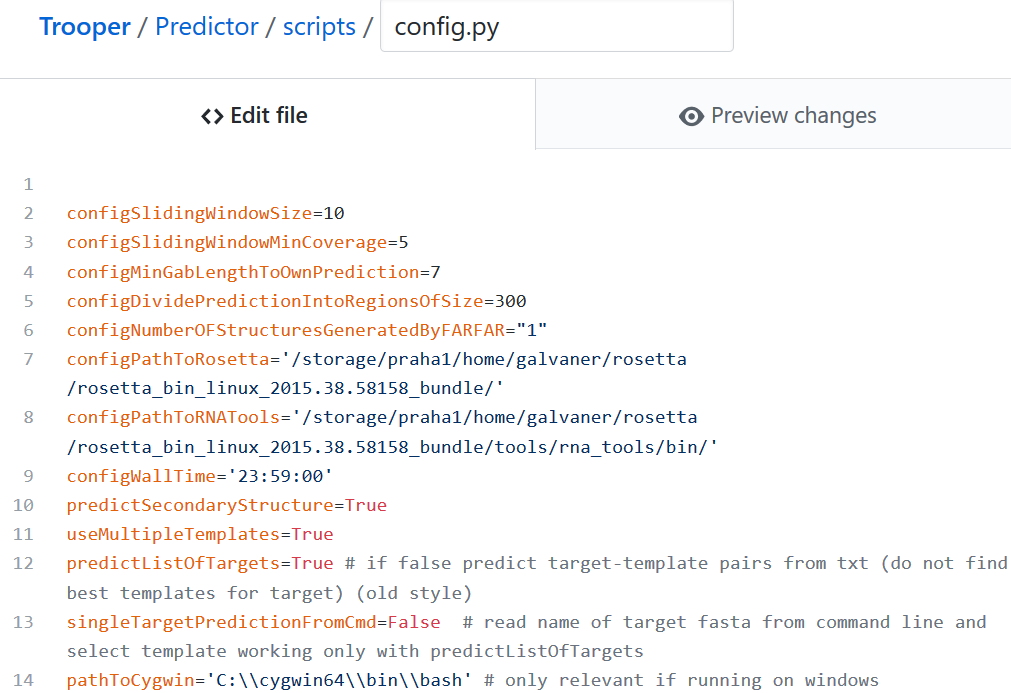
\includegraphics[width=\textwidth]{../img/config}
\caption{Príklad konfiguračného súboru.}
\label{obr04:config}
\end{figure}


\indent Kroky potrebné vykonať pre kompletnú predikciu štruktúry:
\begin{enumerate}
\item Dodať vstupný súbor target template párov
\item Uistiť sa, že potrebné pdb a fasta súbory sa nachádzajú v rovnomenných priečinkoch.
\item Spustiť skript prepare\_rosetta\_prediction.sh a uistiť sa, že dobehol.
\item Spustiť skript startFARFAR.sh.
\item Počkať, kým predikcia nekonzervovaných úsekov dobehne.
\item Spustiť skript extract\_pdbs.sh.
\item Spustiť skript concat\_pdbs.sh
\end{enumerate}

\indent Pre otestovanie algoritmu sme použili všetky stiahnuté štruktúry sekvencie dĺžky 50 a viac nukleotidov. Najprv sme ich rozdelili do priehradok podľa dĺžky (50-100nt, 101-500nt, 500-viac nt). Štruktúry v priehradkách sme následne spárovali každú s každou ako target - template dvojice a tieto dvojice rozdelili do skupín podľa podobnosti a pomeru medzier vzhľadom na zarovnanie \ref{tab4.1}. Z bakalárskej práce sme vedeli, že predikovať sekvenciu na základe štruktúry s podobnosťou menšou ako 60\% nie je vhodné, čo sa nám potvrdilo aj pri tomto pokuse. Naopak, pri podobností sekvencií väčšej ako 60\% sme schopní dosahovať presnosť predikcie okolo 10Å. Tieto výsledky sme publikovali v článku \cite{7822808}. 

\begin{table}[b!]
\centering
\begin{tabular}{cccc}
\toprule
Podobnosť (\%) & Gap (\%)  & Priemer RMSD (Å) & Smerodatná odchýlka  (Å)\\
\midrule
30-45  & 30-45 & 32,05 & 6,09 \\
45-60  & 30-45 & 32,30 & 4,78 \\
60-75  &   0-15 & 11,88 & 7,81 \\
60-75  & 15-30 &   9,63 & 2,33 \\
60-75  & 30-45 &   8,80 & 7,20 \\
75-90  &   0-15 &   6,02 & 4,37 \\
75-90  & 15-30 &   6,93 & 4,45 \\
\bottomrule
\end{tabular}
\caption{Výsledky predikcie pre target template páry dĺžky 50-500 nukleotidov. }\label{tab4.1}
\end{table}


\section{Porovnanie s ModeRNA}
V bakalárskej práci, sme algoritmus porovnávali s algortimom FARFAR,  ktorý z princípu nedokáže v rozumnom čase predikovať dlhšie štruktúry. Teraz sme sa rozhodli porovnať náš algoritmus s komparatívnou predikciou ModeRNA. Pre porovnanie sme sa rozhodli napredikovať rovnaké sekvencie za pomoci rovnakých target štruktúr a porovnať  výsledky z ModeRNA s výsledkami nášho algoritmu. Napísali sme skript ModeRNA/moderRNA.py, ktorý sa pokúša predikovať target - template páry poskytuté na vstupe. Predikcia v ModeRNA je výrazne rýchlejšia a vytvorenie jednej štruktúry sa väčšinou pohybuje v rádoch minút. Výsledky oboch algoritmov sme porovnali \ref{tab4.2}, pričom sme uvažovali iba predikcie, ktoré úspešne vytvorili oba algoritmy. V tomto prípade sme rozlišovali dĺžky štruktúr a to 50-100 nukleotidov a 101-500 nukleotidov. Kritérium na podobnosť tempate štruktúry bolo pre všetky dĺžky rovnaké, a to 60-90\%. Z výsledkov vidno, že ModeRNA bola úspešnejšia v predikovaní dlhších štruktúr, pričom naopak náš algoritmus si viedol lepšie pri predikovaní kratších štruktúr. Na druhej strane ModeRNA dokázala napredikovať celkovo viac štruktúr oproti našemu algoritmu, pretože dokázala lepšie zvládnuť nedokonalé vstupné dáta.

\begin{table}[b!]
\centering
\begin{tabular}{ccc}
\toprule
Dĺžka (nt) & ModeRNA RMSD (Å) & Trooper RMSD (Å) \\
\midrule
50-100    & 5,77 & 8,34  \\
101-500  & 8,25 & 4,29  \\
\bottomrule
50-500  & 6,21 & 7,65  \\
\end{tabular}
\caption{Porovnanie našeho algoritmu s ModeRNA. }\label{tab4.2}
\end{table}

\section{Porovnanie predikcie dlhých štruktúr s ModeRNA}
Algoritmy založené na princípe komparatívneho modelovania majú vďaka vysoko konzervovaným ribozomálnym RNA štruktúram potenciál predikovať prakticky neobmedzene dlhé štruktúry, ak pre ne existuje dosť dobrá template štruktúra. Predikcia štruktúr dlhých niekoľko tisic nukleotidov samozrejme prináša problémy ako dlhšie nekonzervované úseky a celkovo dlhší čas predikcie. Skúšali sme predikovať 4 rôzne target-template páry aj pomocou nášho algoritmu aj pomocou ModeRNA algoritmu. Pravdepodobne kvôli tomu, že ModeRNA používa na vyplnenie nekonzervovaných úsekov knižnicu fragmentov, sa v takto dlhej štruktúre našiel nekonzervovaný úsek, ktorý ModeRNA nedokázala napredikovať. Náš algoritmus má síce s dlhými úsekmi problémy tiež, ale vďaka ich de novo predikcií dokázal napredikovať aj takýto úsek \ref{tab4.3}.

\begin{table}[b!]
\centering
\begin{tabular}{ccccc}
\toprule
Target(len) & Template(len) & Sim(\%) & Trooper & ModeRNA\\
\midrule
3DG0(2904)  & 2O45(2880) & 68  & 13,65 & No fragments candidates.\\
4JI1(1522)  & 4V4Q(1542) & 71,6  & 14,5 &  No fragments candidates.\\
4V6W(1995)  &  4V6X(1869) & 68,3  & 32,7 & Sequences do not match.\\
3DG5(1542)  & 3J2G(1533) &  99,4  & 9,6 & 9,6\\
\bottomrule
\end{tabular}
\caption{Porovnanie výsledkov predikcie vybraných dlhých štruktúr pomocou našeho algoritmu a pomocou ModeRNA. }\label{tab4.3}
\end{table}


\section{Úprava vstupných dát}
Fasta a pdb súbory sme stiahli zo stránok ProteinDataBank \url{https://www.rcsb.org} \cite{PDB00}. Sú to experimentálne získane štruktúry, ktoré často nie sú kompletné, alebo obsahujú chyby. Problém pre náš algoritmus nastáva hlavne v prípade, kedy sekvencia fasta súboru nesedí so sekvenciou extrahovanou z pdb súboru. Takto upravené vstupné data sme použíali na testovanie posledného vylepšenia algoritmu, teda s použitím viacerých template štruktúr. Generovanie je naimplementované v priečinku s relatívnou cestou Predictor/MyTools/CreateFastasFromPdb.


\indent Principiálne problémy s rozdielnymi sekvenciami v nášom algoritme nastávajú v troch konkrétnych prípadoch: 

\begin{enumerate}
\item Pri hľadaní vhodnej template štruktúry pre predikciu (funkcionalita automatického vyhľadávanie template štruktúry).
\item Pri mapovaní temlate štruktúry na konzervované úseky plynúce zo zarovnania sekvencií. \ref{3-map}
\item Pri hľadaní a mapovaní sekundárných template štruktúr. 
\end{enumerate}


\indent V prípade že nastane takáto situácia algoritmus nedokáže pokračovať v predikcií. Preto sme to doteraz riešili tak, že sme sa pokúsili template fasta sekvenciu posunúť pridaním dummy reziduí na jej začiatok (predpoklad, že z FASTA sekvencie chýba na začiatku pár reziduí a ďalej sa už bude poradie nukleotidov zhodovať s tým v pdb súbore) a v prípade, že sa nám niečo takéto nepodarilo nájsť danú štruktúru sme ako template nepoužili.


\indent Rozhodli sme sa skúsiť eliminovať tento problém tak, že sme si vygenerovali fasta sekvencie z pdb súborov. Tu ale nastáva problém s častou nekompletnosťou pdb súborov, kedy býva časté, že začiatok, prípadne koniec štruktúry chýba. Chýbajúce úseky znova nahradzujeme dummy reziduami (písmeno X). Takéto štruktúry môžu byť následne bez problémov použité ako template alebo sekundárny template pri predikcii, pretože pridaný dummy nukleotid X sa nezarovná na target sekvenciu a bude neskôr dopredikovaný. Z princípu sekencia obsahujúca takéto dummy nukleotidy nemôže byť predikovaná, pretože nevieme, aký nukleotid máme na dané miesto vlastne predikovať.


\indent Okrem problému s mapovaním štruktúry a sekvencie sme riešili aj duplicitu rôzne pomenovaných, ale pritom rovnakých štruktúr. V pôvodnej implementácií nám to nerobilo problém, pretože sme si dopredu testovacie dáta rozdelili podľa podobností zarovnaní ich sekvencií a tie vzájomne spárovali. Teda ako template sme používali len dosť odlišné template sekvencie od target sekvencie, nakoľko predikovať sekvenciu pomocou inej so skoro 100\% zhodou by bolo triviálne. V prípade, že hľadáme vhodný template sa však chceme vyhnúť zbytočnému zarovnávaniu sekvencií a preto sme pri generovaní fasta súborov rovno podobné odfiltrujeme. Docielime to jednoducho tak, že pri vygenerovaní novej fasta sekvencie ju globálne zarovnáme na všetky už vygenerované fasta sekvencie a ak podobnosť presiahne istú konštantnú hranicu (použíli sme 97,5\%), tak takúto sekvenciu nepridáme, medzi už vygenerované sekvencie.